% Generated by Sphinx.
\def\sphinxdocclass{report}
\documentclass[letterpaper,10pt,english]{sphinxmanual}
\usepackage[utf8]{inputenc}
\DeclareUnicodeCharacter{00A0}{\nobreakspace}
\usepackage[T1]{fontenc}
\usepackage{babel}
\usepackage{times}
\usepackage[Bjarne]{fncychap}
\usepackage{longtable}
\usepackage{sphinx}
\usepackage{multirow}


\title{Pynoramix Documentation}
\date{June 25, 2012}
\release{0.1}
\author{Diego Prada-Gracia}
\newcommand{\sphinxlogo}{}
\renewcommand{\releasename}{Release}
\makeindex

\makeatletter
\def\PYG@reset{\let\PYG@it=\relax \let\PYG@bf=\relax%
    \let\PYG@ul=\relax \let\PYG@tc=\relax%
    \let\PYG@bc=\relax \let\PYG@ff=\relax}
\def\PYG@tok#1{\csname PYG@tok@#1\endcsname}
\def\PYG@toks#1+{\ifx\relax#1\empty\else%
    \PYG@tok{#1}\expandafter\PYG@toks\fi}
\def\PYG@do#1{\PYG@bc{\PYG@tc{\PYG@ul{%
    \PYG@it{\PYG@bf{\PYG@ff{#1}}}}}}}
\def\PYG#1#2{\PYG@reset\PYG@toks#1+\relax+\PYG@do{#2}}

\def\PYG@tok@gd{\def\PYG@tc##1{\textcolor[rgb]{0.63,0.00,0.00}{##1}}}
\def\PYG@tok@gu{\let\PYG@bf=\textbf\def\PYG@tc##1{\textcolor[rgb]{0.50,0.00,0.50}{##1}}}
\def\PYG@tok@gt{\def\PYG@tc##1{\textcolor[rgb]{0.00,0.25,0.82}{##1}}}
\def\PYG@tok@gs{\let\PYG@bf=\textbf}
\def\PYG@tok@gr{\def\PYG@tc##1{\textcolor[rgb]{1.00,0.00,0.00}{##1}}}
\def\PYG@tok@cm{\let\PYG@it=\textit\def\PYG@tc##1{\textcolor[rgb]{0.25,0.50,0.56}{##1}}}
\def\PYG@tok@vg{\def\PYG@tc##1{\textcolor[rgb]{0.73,0.38,0.84}{##1}}}
\def\PYG@tok@m{\def\PYG@tc##1{\textcolor[rgb]{0.13,0.50,0.31}{##1}}}
\def\PYG@tok@mh{\def\PYG@tc##1{\textcolor[rgb]{0.13,0.50,0.31}{##1}}}
\def\PYG@tok@cs{\def\PYG@tc##1{\textcolor[rgb]{0.25,0.50,0.56}{##1}}\def\PYG@bc##1{\colorbox[rgb]{1.00,0.94,0.94}{##1}}}
\def\PYG@tok@ge{\let\PYG@it=\textit}
\def\PYG@tok@vc{\def\PYG@tc##1{\textcolor[rgb]{0.73,0.38,0.84}{##1}}}
\def\PYG@tok@il{\def\PYG@tc##1{\textcolor[rgb]{0.13,0.50,0.31}{##1}}}
\def\PYG@tok@go{\def\PYG@tc##1{\textcolor[rgb]{0.19,0.19,0.19}{##1}}}
\def\PYG@tok@cp{\def\PYG@tc##1{\textcolor[rgb]{0.00,0.44,0.13}{##1}}}
\def\PYG@tok@gi{\def\PYG@tc##1{\textcolor[rgb]{0.00,0.63,0.00}{##1}}}
\def\PYG@tok@gh{\let\PYG@bf=\textbf\def\PYG@tc##1{\textcolor[rgb]{0.00,0.00,0.50}{##1}}}
\def\PYG@tok@ni{\let\PYG@bf=\textbf\def\PYG@tc##1{\textcolor[rgb]{0.84,0.33,0.22}{##1}}}
\def\PYG@tok@nl{\let\PYG@bf=\textbf\def\PYG@tc##1{\textcolor[rgb]{0.00,0.13,0.44}{##1}}}
\def\PYG@tok@nn{\let\PYG@bf=\textbf\def\PYG@tc##1{\textcolor[rgb]{0.05,0.52,0.71}{##1}}}
\def\PYG@tok@no{\def\PYG@tc##1{\textcolor[rgb]{0.38,0.68,0.84}{##1}}}
\def\PYG@tok@na{\def\PYG@tc##1{\textcolor[rgb]{0.25,0.44,0.63}{##1}}}
\def\PYG@tok@nb{\def\PYG@tc##1{\textcolor[rgb]{0.00,0.44,0.13}{##1}}}
\def\PYG@tok@nc{\let\PYG@bf=\textbf\def\PYG@tc##1{\textcolor[rgb]{0.05,0.52,0.71}{##1}}}
\def\PYG@tok@nd{\let\PYG@bf=\textbf\def\PYG@tc##1{\textcolor[rgb]{0.33,0.33,0.33}{##1}}}
\def\PYG@tok@ne{\def\PYG@tc##1{\textcolor[rgb]{0.00,0.44,0.13}{##1}}}
\def\PYG@tok@nf{\def\PYG@tc##1{\textcolor[rgb]{0.02,0.16,0.49}{##1}}}
\def\PYG@tok@si{\let\PYG@it=\textit\def\PYG@tc##1{\textcolor[rgb]{0.44,0.63,0.82}{##1}}}
\def\PYG@tok@s2{\def\PYG@tc##1{\textcolor[rgb]{0.25,0.44,0.63}{##1}}}
\def\PYG@tok@vi{\def\PYG@tc##1{\textcolor[rgb]{0.73,0.38,0.84}{##1}}}
\def\PYG@tok@nt{\let\PYG@bf=\textbf\def\PYG@tc##1{\textcolor[rgb]{0.02,0.16,0.45}{##1}}}
\def\PYG@tok@nv{\def\PYG@tc##1{\textcolor[rgb]{0.73,0.38,0.84}{##1}}}
\def\PYG@tok@s1{\def\PYG@tc##1{\textcolor[rgb]{0.25,0.44,0.63}{##1}}}
\def\PYG@tok@gp{\let\PYG@bf=\textbf\def\PYG@tc##1{\textcolor[rgb]{0.78,0.36,0.04}{##1}}}
\def\PYG@tok@sh{\def\PYG@tc##1{\textcolor[rgb]{0.25,0.44,0.63}{##1}}}
\def\PYG@tok@ow{\let\PYG@bf=\textbf\def\PYG@tc##1{\textcolor[rgb]{0.00,0.44,0.13}{##1}}}
\def\PYG@tok@sx{\def\PYG@tc##1{\textcolor[rgb]{0.78,0.36,0.04}{##1}}}
\def\PYG@tok@bp{\def\PYG@tc##1{\textcolor[rgb]{0.00,0.44,0.13}{##1}}}
\def\PYG@tok@c1{\let\PYG@it=\textit\def\PYG@tc##1{\textcolor[rgb]{0.25,0.50,0.56}{##1}}}
\def\PYG@tok@kc{\let\PYG@bf=\textbf\def\PYG@tc##1{\textcolor[rgb]{0.00,0.44,0.13}{##1}}}
\def\PYG@tok@c{\let\PYG@it=\textit\def\PYG@tc##1{\textcolor[rgb]{0.25,0.50,0.56}{##1}}}
\def\PYG@tok@mf{\def\PYG@tc##1{\textcolor[rgb]{0.13,0.50,0.31}{##1}}}
\def\PYG@tok@err{\def\PYG@bc##1{\fcolorbox[rgb]{1.00,0.00,0.00}{1,1,1}{##1}}}
\def\PYG@tok@kd{\let\PYG@bf=\textbf\def\PYG@tc##1{\textcolor[rgb]{0.00,0.44,0.13}{##1}}}
\def\PYG@tok@ss{\def\PYG@tc##1{\textcolor[rgb]{0.32,0.47,0.09}{##1}}}
\def\PYG@tok@sr{\def\PYG@tc##1{\textcolor[rgb]{0.14,0.33,0.53}{##1}}}
\def\PYG@tok@mo{\def\PYG@tc##1{\textcolor[rgb]{0.13,0.50,0.31}{##1}}}
\def\PYG@tok@mi{\def\PYG@tc##1{\textcolor[rgb]{0.13,0.50,0.31}{##1}}}
\def\PYG@tok@kn{\let\PYG@bf=\textbf\def\PYG@tc##1{\textcolor[rgb]{0.00,0.44,0.13}{##1}}}
\def\PYG@tok@o{\def\PYG@tc##1{\textcolor[rgb]{0.40,0.40,0.40}{##1}}}
\def\PYG@tok@kr{\let\PYG@bf=\textbf\def\PYG@tc##1{\textcolor[rgb]{0.00,0.44,0.13}{##1}}}
\def\PYG@tok@s{\def\PYG@tc##1{\textcolor[rgb]{0.25,0.44,0.63}{##1}}}
\def\PYG@tok@kp{\def\PYG@tc##1{\textcolor[rgb]{0.00,0.44,0.13}{##1}}}
\def\PYG@tok@w{\def\PYG@tc##1{\textcolor[rgb]{0.73,0.73,0.73}{##1}}}
\def\PYG@tok@kt{\def\PYG@tc##1{\textcolor[rgb]{0.56,0.13,0.00}{##1}}}
\def\PYG@tok@sc{\def\PYG@tc##1{\textcolor[rgb]{0.25,0.44,0.63}{##1}}}
\def\PYG@tok@sb{\def\PYG@tc##1{\textcolor[rgb]{0.25,0.44,0.63}{##1}}}
\def\PYG@tok@k{\let\PYG@bf=\textbf\def\PYG@tc##1{\textcolor[rgb]{0.00,0.44,0.13}{##1}}}
\def\PYG@tok@se{\let\PYG@bf=\textbf\def\PYG@tc##1{\textcolor[rgb]{0.25,0.44,0.63}{##1}}}
\def\PYG@tok@sd{\let\PYG@it=\textit\def\PYG@tc##1{\textcolor[rgb]{0.25,0.44,0.63}{##1}}}

\def\PYGZbs{\char`\\}
\def\PYGZus{\char`\_}
\def\PYGZob{\char`\{}
\def\PYGZcb{\char`\}}
\def\PYGZca{\char`\^}
% for compatibility with earlier versions
\def\PYGZat{@}
\def\PYGZlb{[}
\def\PYGZrb{]}
\makeatother

\begin{document}

\maketitle
\tableofcontents
\phantomsection\label{index::doc}


Contents:


\chapter{Getting Started}
\label{getting_started:getting-started}\label{getting_started::doc}\label{getting_started:welcome-to-pynoramix-s-documentation}

\section{Getting Pynoramix}
\label{getting_started:getting-pynoramix}

\subsection{Last stable version (0.1)}
\label{getting_started:last-stable-version-0-1}
-Adding the project in easy\_install or setup.py (\href{http://packages.python.org/an\_example\_pypi\_project/setuptools.html\#registering-your-project}{http://packages.python.org/an\_example\_pypi\_project/setuptools.html\#registering-your-project})

-Links to raolab.com or GitHub from raolab.


\subsection{Source Code}
\label{getting_started:source-code}
Document the project in GitHub and add the link.


\section{Installing}
\label{getting_started:installing}
Pynoramix depends on some packages:
\begin{itemize}
\item {} 
NumPy

\end{itemize}


\chapter{Getting started}
\label{getting_started_ex:getting-started}\label{getting_started_ex::doc}\label{getting_started_ex:id1}

\section{Installing your doc directory}
\label{getting_started_ex:installing-your-doc-directory}\label{getting_started_ex:installing-docdir}
You may already have sphinx \href{http://sphinx.pocoo.org/}{sphinx}
installed -- you can check by doing:

\begin{Verbatim}[commandchars=\\\{\}]
python -c 'import sphinx'
\end{Verbatim}

If that fails grab the latest version of and install it with:

\begin{Verbatim}[commandchars=\\\{\}]
\textgreater{} sudo easy\_install -U Sphinx
\end{Verbatim}

Now you are ready to build a template for your docs, using
sphinx-quickstart:

\begin{Verbatim}[commandchars=\\\{\}]
\textgreater{} sphinx-quickstart
\end{Verbatim}

accepting most of the defaults.  I choose ``sampledoc'' as the name of my
project.  cd into your new directory and check the contents:

\begin{Verbatim}[commandchars=\\\{\}]
home:\textasciitilde{}/tmp/sampledoc\textgreater{} ls
Makefile      \_static         conf.py
\_build                \_templates      index.rst
\end{Verbatim}

The index.rst is the master ReST for your project, but before adding
anything, let's see if we can build some html:

\begin{Verbatim}[commandchars=\\\{\}]
make html
\end{Verbatim}

If you now point your browser to \code{\_build/html/index.html}, you
should see a basic sphinx site.

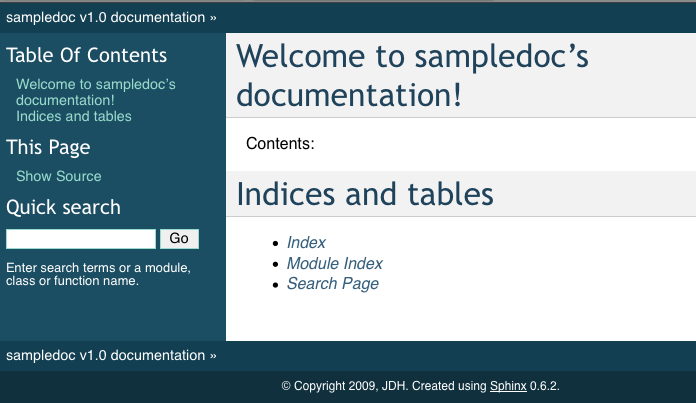
\includegraphics{basic_screenshot.png}


\subsection{Fetching the data}
\label{getting_started_ex:id2}\label{getting_started_ex:fetching-the-data}
Now we will start to customize out docs.  Grab a couple of files from
the \href{http://matplotlib.svn.sourceforge.net/viewvc/matplotlib/trunk/sampledoc\_tut/}{web site}
or svn.  You will need \code{getting\_started.rst} and
\code{\_static/basic\_screenshot.png}.  All of the files live in the
``completed'' version of this tutorial, but since this is a tutorial,
we'll just grab them one at a time, so you can learn what needs to be
changed where.  Since we have more files to come, I'm going to grab
the whole svn directory and just copy the files I need over for now.
First, I'll cd up back into the directory containing my project, check
out the ``finished'' product from svn, and then copy in just the files I
need into my \code{sampledoc} directory:

\begin{Verbatim}[commandchars=\\\{\}]
home:\textasciitilde{}/tmp/sampledoc\textgreater{} pwd
/Users/jdhunter/tmp/sampledoc
home:\textasciitilde{}/tmp/sampledoc\textgreater{} cd ..
home:\textasciitilde{}/tmp\textgreater{} svn co https://matplotlib.svn.sourceforge.net/svnroot/\PYGZbs{}
matplotlib/trunk/sampledoc\_tut
A    sampledoc\_tut/cheatsheet.rst
A    sampledoc\_tut/\_static
A    sampledoc\_tut/\_static/basic\_screenshot.png
A    sampledoc\_tut/conf.py
A    sampledoc\_tut/Makefile
A    sampledoc\_tut/\_templates
A    sampledoc\_tut/\_build
A    sampledoc\_tut/getting\_started.rst
A    sampledoc\_tut/index.rst
Checked out revision 7449.
home:\textasciitilde{}/tmp\textgreater{} cp sampledoc\_tut/getting\_started.rst sampledoc/
home:\textasciitilde{}/tmp\textgreater{} cp sampledoc\_tut/\_static/basic\_screenshot.png \PYGZbs{}
sampledoc/\_static/
\end{Verbatim}

The last step is to modify \code{index.rst} to include the
\code{getting\_started.rst} file (be careful with the indentation, the
``g'' in ``getting\_started'' should line up with the `:' in \code{:maxdepth}:

\begin{Verbatim}[commandchars=\\\{\}]
Contents:

.. toctree::
   :maxdepth: 2

   getting\_started.rst
\end{Verbatim}

and then rebuild the docs:

\begin{Verbatim}[commandchars=\\\{\}]
cd sampledoc
make html
\end{Verbatim}

When you reload the page by refreshing your browser pointing to
\code{\_build/html/index.html}, you should see a link to the
``Getting Started'' docs, and in there this page with the screenshot.
\emph{Voila!}

Note we used the image directive to include to the screenshot above
with:

\begin{Verbatim}[commandchars=\\\{\}]
.. image:: \_static/basic\_screenshot.png
\end{Verbatim}

Next we'll customize the look and feel of our site to give it a logo,
some custom css, and update the navigation panels to look more like
the \href{http://sphinx.pocoo.org/}{sphinx} site itself -- see
\emph{custom\_look}.


\chapter{Tutorials and Examples}
\label{tutorial_examples:tutorials-and-examples}\label{tutorial_examples::doc}
First of all, lets load Pynoramix in our script or in a ipython session:

\begin{Verbatim}[commandchars=\\\{\}]
\PYG{g+gp}{In [1]: }\PYG{k+kn}{from} \PYG{n+nn}{pynoramix\PYGZus{}beta} \PYG{k+kn}{import} \PYG{o}{*}
\end{Verbatim}

Some basic notions on python will be assumed along this tutorial. If you just landed here without any idea on python, have a look to the section \emph{First steps on python}.

\begin{notice}{note}{Todo}

Make a short tutorial on python, enough to run pynoramix.
\end{notice}


\bigskip\hrule{}\bigskip



\section{Networks}
\label{tutorial_examples:networks}
How to create, load and handle a network.


\subsection{A network from scratch}
\label{tutorial_examples:a-network-from-scratch}
Lets create as simple example a network of cities:

\begin{Verbatim}[commandchars=\\\{\}]
\PYG{g+gp}{In [2]: }\PYG{n}{cities}\PYG{o}{=}\PYG{n}{net}\PYG{p}{(}\PYG{p}{)}
\PYG{c}{\# Network:}
\PYG{c}{\# 0 nodes}
\PYG{c}{\# 0 links out}
\PYG{c}{\# 0 total weight nodes}
\end{Verbatim}

Nodes can be added in two ways, along or inferred by the links addition:

\begin{Verbatim}[commandchars=\\\{\}]
\PYG{g+gp}{In [3]: }\PYG{n}{cities}\PYG{o}{.}\PYG{n}{add\PYGZus{}node}\PYG{p}{(}\PYG{l+s}{'}\PYG{l+s}{Zaragoza}\PYG{l+s}{'}\PYG{p}{)}
\PYG{g+gp}{In [4]: }\PYG{n}{cities}\PYG{o}{.}\PYG{n}{add\PYGZus{}link}\PYG{p}{(}\PYG{l+s}{'}\PYG{l+s}{Rome}\PYG{l+s}{'}\PYG{p}{,}\PYG{l+s}{'}\PYG{l+s}{Turin}\PYG{l+s}{'}\PYG{p}{,}\PYG{l+m+mi}{446}\PYG{p}{)}
\PYG{g+gp}{In [5]: }\PYG{n}{cities}\PYG{o}{.}\PYG{n}{add\PYGZus{}link}\PYG{p}{(}\PYG{l+s}{'}\PYG{l+s}{Rome}\PYG{l+s}{'}\PYG{p}{,}\PYG{l+s}{'}\PYG{l+s}{Zaragoza}\PYG{l+s}{'}\PYG{p}{,}\PYG{l+m+mi}{1112}\PYG{p}{)}
\PYG{g+gp}{In [6]: }\PYG{n}{cities}\PYG{o}{.}\PYG{n}{add\PYGZus{}link}\PYG{p}{(}\PYG{l+s}{'}\PYG{l+s}{Zaragoza}\PYG{l+s}{'}\PYG{p}{,}\PYG{l+s}{'}\PYG{l+s}{Kiev}\PYG{l+s}{'}\PYG{p}{,}\PYG{l+m+mi}{2561}\PYG{p}{)}
\PYG{g+gp}{In [7]: }\PYG{n}{cities}\PYG{o}{.}\PYG{n}{info}\PYG{p}{(}\PYG{p}{)}
\PYG{c}{\# Network:}
\PYG{c}{\# 4 nodes}
\PYG{c}{\# 3 links out}
\PYG{c}{\# 0 total weight nodes}
\end{Verbatim}

The nodes are attached to the network in order of creation:

\begin{Verbatim}[commandchars=\\\{\}]
\PYG{g+gp}{In [7]: }\PYG{n}{cities}\PYG{o}{.}\PYG{n}{node}\PYG{p}{[}\PYG{l+m+mi}{0}\PYG{p}{]}\PYG{o}{.}\PYG{n}{label}
\PYG{g+gr}{Out[7]: }\PYG{l+s}{'}\PYG{l+s}{Zaragoza}\PYG{l+s}{'}
\PYG{g+gp}{In [8]: }\PYG{n}{cities}\PYG{o}{.}\PYG{n}{node}\PYG{p}{[}\PYG{l+m+mi}{3}\PYG{p}{]}\PYG{o}{.}\PYG{n}{label}
\PYG{g+gr}{Out[8]: }\PYG{l+s}{'}\PYG{l+s}{Kiev}\PYG{l+s}{'}
\end{Verbatim}

Links are stored as a dictionary for each node (see ref). Nodes are from now on referred because of their indexes.

\begin{Verbatim}[commandchars=\\\{\}]
\PYG{g+gp}{In [9]: }\PYG{n}{cities}\PYG{o}{.}\PYG{n}{labels}\PYG{p}{[}\PYG{l+s}{'}\PYG{l+s}{Rome}\PYG{l+s}{'}\PYG{p}{]}
\PYG{g+gr}{Out[9]: }\PYG{l+m+mi}{1}
\PYG{g+gp}{In [10]: }\PYG{n}{cities}\PYG{o}{.}\PYG{n}{node}\PYG{p}{[}\PYG{l+m+mi}{1}\PYG{p}{]}\PYG{o}{.}\PYG{n}{link}\PYG{o}{.}\PYG{n}{keys}\PYG{p}{(}\PYG{p}{)}
\PYG{g+gr}{Out[10]: }\PYG{p}{[}\PYG{l+m+mi}{0}\PYG{p}{,} \PYG{l+m+mi}{2}\PYG{p}{]}
\PYG{g+gp}{In [11]: }\PYG{k}{print} \PYG{l+s}{'}\PYG{l+s}{From Rome to Zaragoza: }\PYG{l+s}{'}\PYG{p}{,} \PYG{n}{cities}\PYG{o}{.}\PYG{n}{node}\PYG{p}{[}\PYG{l+m+mi}{1}\PYG{p}{]}\PYG{o}{.}\PYG{n}{link}\PYG{p}{[}\PYG{l+m+mi}{0}\PYG{p}{]}\PYG{p}{,} \PYG{l+s}{'}\PYG{l+s}{km.}\PYG{l+s}{'}
\PYG{g+go}{From Rome to Zaragoza:  1112 km.}
\end{Verbatim}


\strong{See Also:}


include here a link to the class definition and attributes.




\subsection{Loading a network from a file}
\label{tutorial_examples:loading-a-network-from-a-file}
A network can be loaded together with their labels. Pynoramix uses its
own compact format for the network, while the labels can be readed with many formats.
This way a network can be initialized with the files or a posteriori:


\chapter{Networks}
\label{networks::doc}\label{networks:networks}
Description of the network object and attributes.
This is a test to include the comments from the code.

nada


\section{Network class}
\label{networks:network-class}\label{networks:module-pyn_cl_net}\index{pyn\_cl\_net (module)}\index{cl\_node (class in pyn\_cl\_net)}

\begin{fulllineitems}
\phantomsection\label{networks:pyn_cl_net.cl_node}\pysigline{\strong{class }\code{pyn\_cl\_net.}\bfcode{cl\_node}}
Fundamental unit to constitute a network together with links.
\begin{quote}\begin{description}
\item[{Variables}] \leavevmode\begin{itemize}
\item {} 
\textbf{label} -- label or key

\item {} 
\textbf{weight} -- weight

\item {} 
\textbf{link} -- linked nodes, \{node\_index, weight\_link\}.

\item {} 
\textbf{k\_out} -- degree or connectivity with directed links out.

\item {} 
\textbf{k\_in} -- degree or connectivity with directed links in.

\item {} 
\textbf{k} -- total degree or connectivity.

\item {} 
\textbf{cluster} -- index of cluster the node belongs to

\item {} 
\textbf{component} -- index of disconnected component the node belongs to

\item {} 
\textbf{coors} -- spatial coordinates for representation

\end{itemize}

\end{description}\end{quote}
\index{most\_weighted\_links() (pyn\_cl\_net.cl\_node method)}

\begin{fulllineitems}
\phantomsection\label{networks:pyn_cl_net.cl_node.most_weighted_links}\pysiglinewithargsret{\bfcode{most\_weighted\_links}}{\emph{length=1}}{}
Ranked indexes of connected nodes according to the weight of the links.
\begin{quote}\begin{description}
\item[{Parameters}] \leavevmode
\textbf{length} (\href{http://docs.python.org/library/functions.html\#int}{\emph{int}}) -- N number of links requested

\item[{Returns}] \leavevmode
ranked node indexes

\item[{Return type}] \leavevmode
N-dim list {[}int{]}

\end{description}\end{quote}

\end{fulllineitems}


\end{fulllineitems}

\index{net (class in pyn\_cl\_net)}

\begin{fulllineitems}
\phantomsection\label{networks:pyn_cl_net.net}\pysiglinewithargsret{\strong{class }\code{pyn\_cl\_net.}\bfcode{net}}{\emph{file\_net=None}, \emph{file\_keys=None}, \emph{directed=True}, \emph{labels\_format=`2columns'}, \emph{verbose=True}}{}
Supra-structure composed by nodes
\index{add\_node() (pyn\_cl\_net.net method)}

\begin{fulllineitems}
\phantomsection\label{networks:pyn_cl_net.net.add_node}\pysiglinewithargsret{\bfcode{add\_node}}{\emph{new\_node}, \emph{weight=0}}{}
Adding a new node to the network.
\begin{quote}\begin{description}
\item[{Parameters}] \leavevmode\begin{itemize}
\item {} 
\textbf{new\_node} (\emph{str,int,float...}) -- key or label of the new node

\item {} 
\textbf{weight} (int, \emph{opt}) -- weight of new node

\end{itemize}

\end{description}\end{quote}

\end{fulllineitems}

\index{info() (pyn\_cl\_net.net method)}

\begin{fulllineitems}
\phantomsection\label{networks:pyn_cl_net.net.info}\pysiglinewithargsret{\bfcode{info}}{}{}
Print network general variables: num\_nodes, k\_total, weight.

\end{fulllineitems}


\end{fulllineitems}


..:param arg1: description
..:param arg2: description
..:type arg1: type description
..:type arg1: type description
..:return: return description
..:rtype: the return type description
..:Example: (followed by a blank line)


\chapter{Ejemplo de Titulo de Capitulo}
\label{example_edition_ex:ejemplo-de-titulo-de-capitulo}\label{example_edition_ex::doc}
There should only be one of these per page and this will also -- when
converting to pdf -- be used for the chapters.


\section{Como itemizo}
\label{example_edition_ex:como-itemizo}
Ejemplos de itemizes.


\subsection{Ejemplos:}
\label{example_edition_ex:ejemplos}
Aqui los ejemplos.


\subsubsection{Ejemplos 1}
\label{example_edition_ex:ejemplos-1}\begin{itemize}
\item {} 
A thing.

\item {} 
Another thing.

\end{itemize}


\subsubsection{Ejemplo 2}
\label{example_edition_ex:ejemplo-2}\begin{enumerate}
\item {} 
Item 1.

\item {} 
Item 2.

\item {} 
Item 3.

\end{enumerate}


\subsubsection{Ejemplo 2}
\label{example_edition_ex:id1}\begin{itemize}
\item {} 
Some.

\item {} 
Thing.

\item {} 
Different.

\end{itemize}


\section{Page Sections}
\label{example_edition_ex:page-sections}
Ejemplos de formato:

\textbf{bold} and \emph{italics}


\section{Marking paragraphs}
\label{example_edition_ex:marking-paragraphs}
This is a statement.

\begin{notice}{warning}{Warning:}
Never, ever, use this code!
\end{notice}
New in version 0.0.1.
It's okay to use this code.

Here is something I want to talk about:

\begin{Verbatim}[commandchars=\\\{\}]
\PYG{k}{def} \PYG{n+nf}{my\PYGZus{}fn}\PYG{p}{(}\PYG{n}{foo}\PYG{p}{,} \PYG{n}{bar}\PYG{o}{=}\PYG{n+nb+bp}{True}\PYG{p}{)}\PYG{p}{:}
    \PYG{l+s+sd}{"""A really useful function.}

\PYG{l+s+sd}{    Returns None}
\PYG{l+s+sd}{    """}
\end{Verbatim}

bla,bla

This is inline \code{if \_\_name\_\_ == '\_\_main\_\_':}


\chapter{Indices and tables}
\label{index:indices-and-tables}\begin{itemize}
\item {} 
\emph{genindex}

\item {} 
\emph{modindex}

\item {} 
\emph{search}

\end{itemize}


\renewcommand{\indexname}{Python Module Index}
\begin{theindex}
\def\bigletter#1{{\Large\sffamily#1}\nopagebreak\vspace{1mm}}
\bigletter{p}
\item {\texttt{pyn\_cl\_net}}, \pageref{networks:module-pyn_cl_net}
\end{theindex}

\renewcommand{\indexname}{Index}
\printindex
\end{document}
